\section{DAC / ADC}

\subsection{Basics}
Resolution: $N$ Bits \\
$Code = \frac{U_{IN}}{U_{FS}} \cdot 2^N$ / $U_{IN} = Code \cdot \frac{U_{FS}}{2^N}$ / $U_{FS} = U_{ref}$ (Single ended) / $U_{FS} = 2 \cdot U_{ref}$ (Differential)\\
$U_{LSB} = \frac{U_{FS}}{2^N}$

\subsection{Noise}
Signal to Noise: $SNR_{db} = 10 \cdot \log_{10}(\frac{P_{signal}}{P_{noise}}) = 20 \cdot \log_{10}(\frac{U_{signal}}{U_{noise}})$\\
Noise due Quantization: $U_{N,RMS} = \frac{U_{LSB}}{\sqrt{12}}$\\
Signal to Noise due Quantization assuming full scale sine input: $SNR_{db} = 1.76 + N \cdot 6.02$\\
Distortion (Based on Fourier series): In: $A_1 \sin(\omega t)$ Out: $A_1 \sin(\omega t) + A_2 \sin(2 \omega t) + \hdots$ $\rightarrow$ $\text{THD} = \sqrt{\frac{A_1^2}{A_2^2 + A_3^2 + \hdots}}$\\
Singnal-to-Noise and Distortion: $SINAD_{db} = 10 \cdot \log_{10}\left(\frac{A_1^2}{P_{noise} + A_2^2 + A_3^2 + \hdots}\right)$\\
Effective Number of Bits: $ENOB = \frac{SINAD_{db} - 1.76}{6.02}$\\
Spurious Free Synamic Range:\\
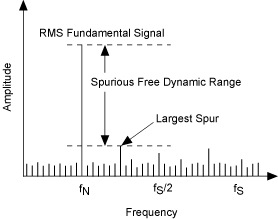
\includegraphics[
		width=0.3\textwidth,
		keepaspectratio,
		angle=0
		]{images/DacAdc/sfdr}

\subsection{Non Lineraries}

\begin{tabular}{m{5cm} m{5cm} m{5cm}}
 	Offset error & Gain Error & \\ 
	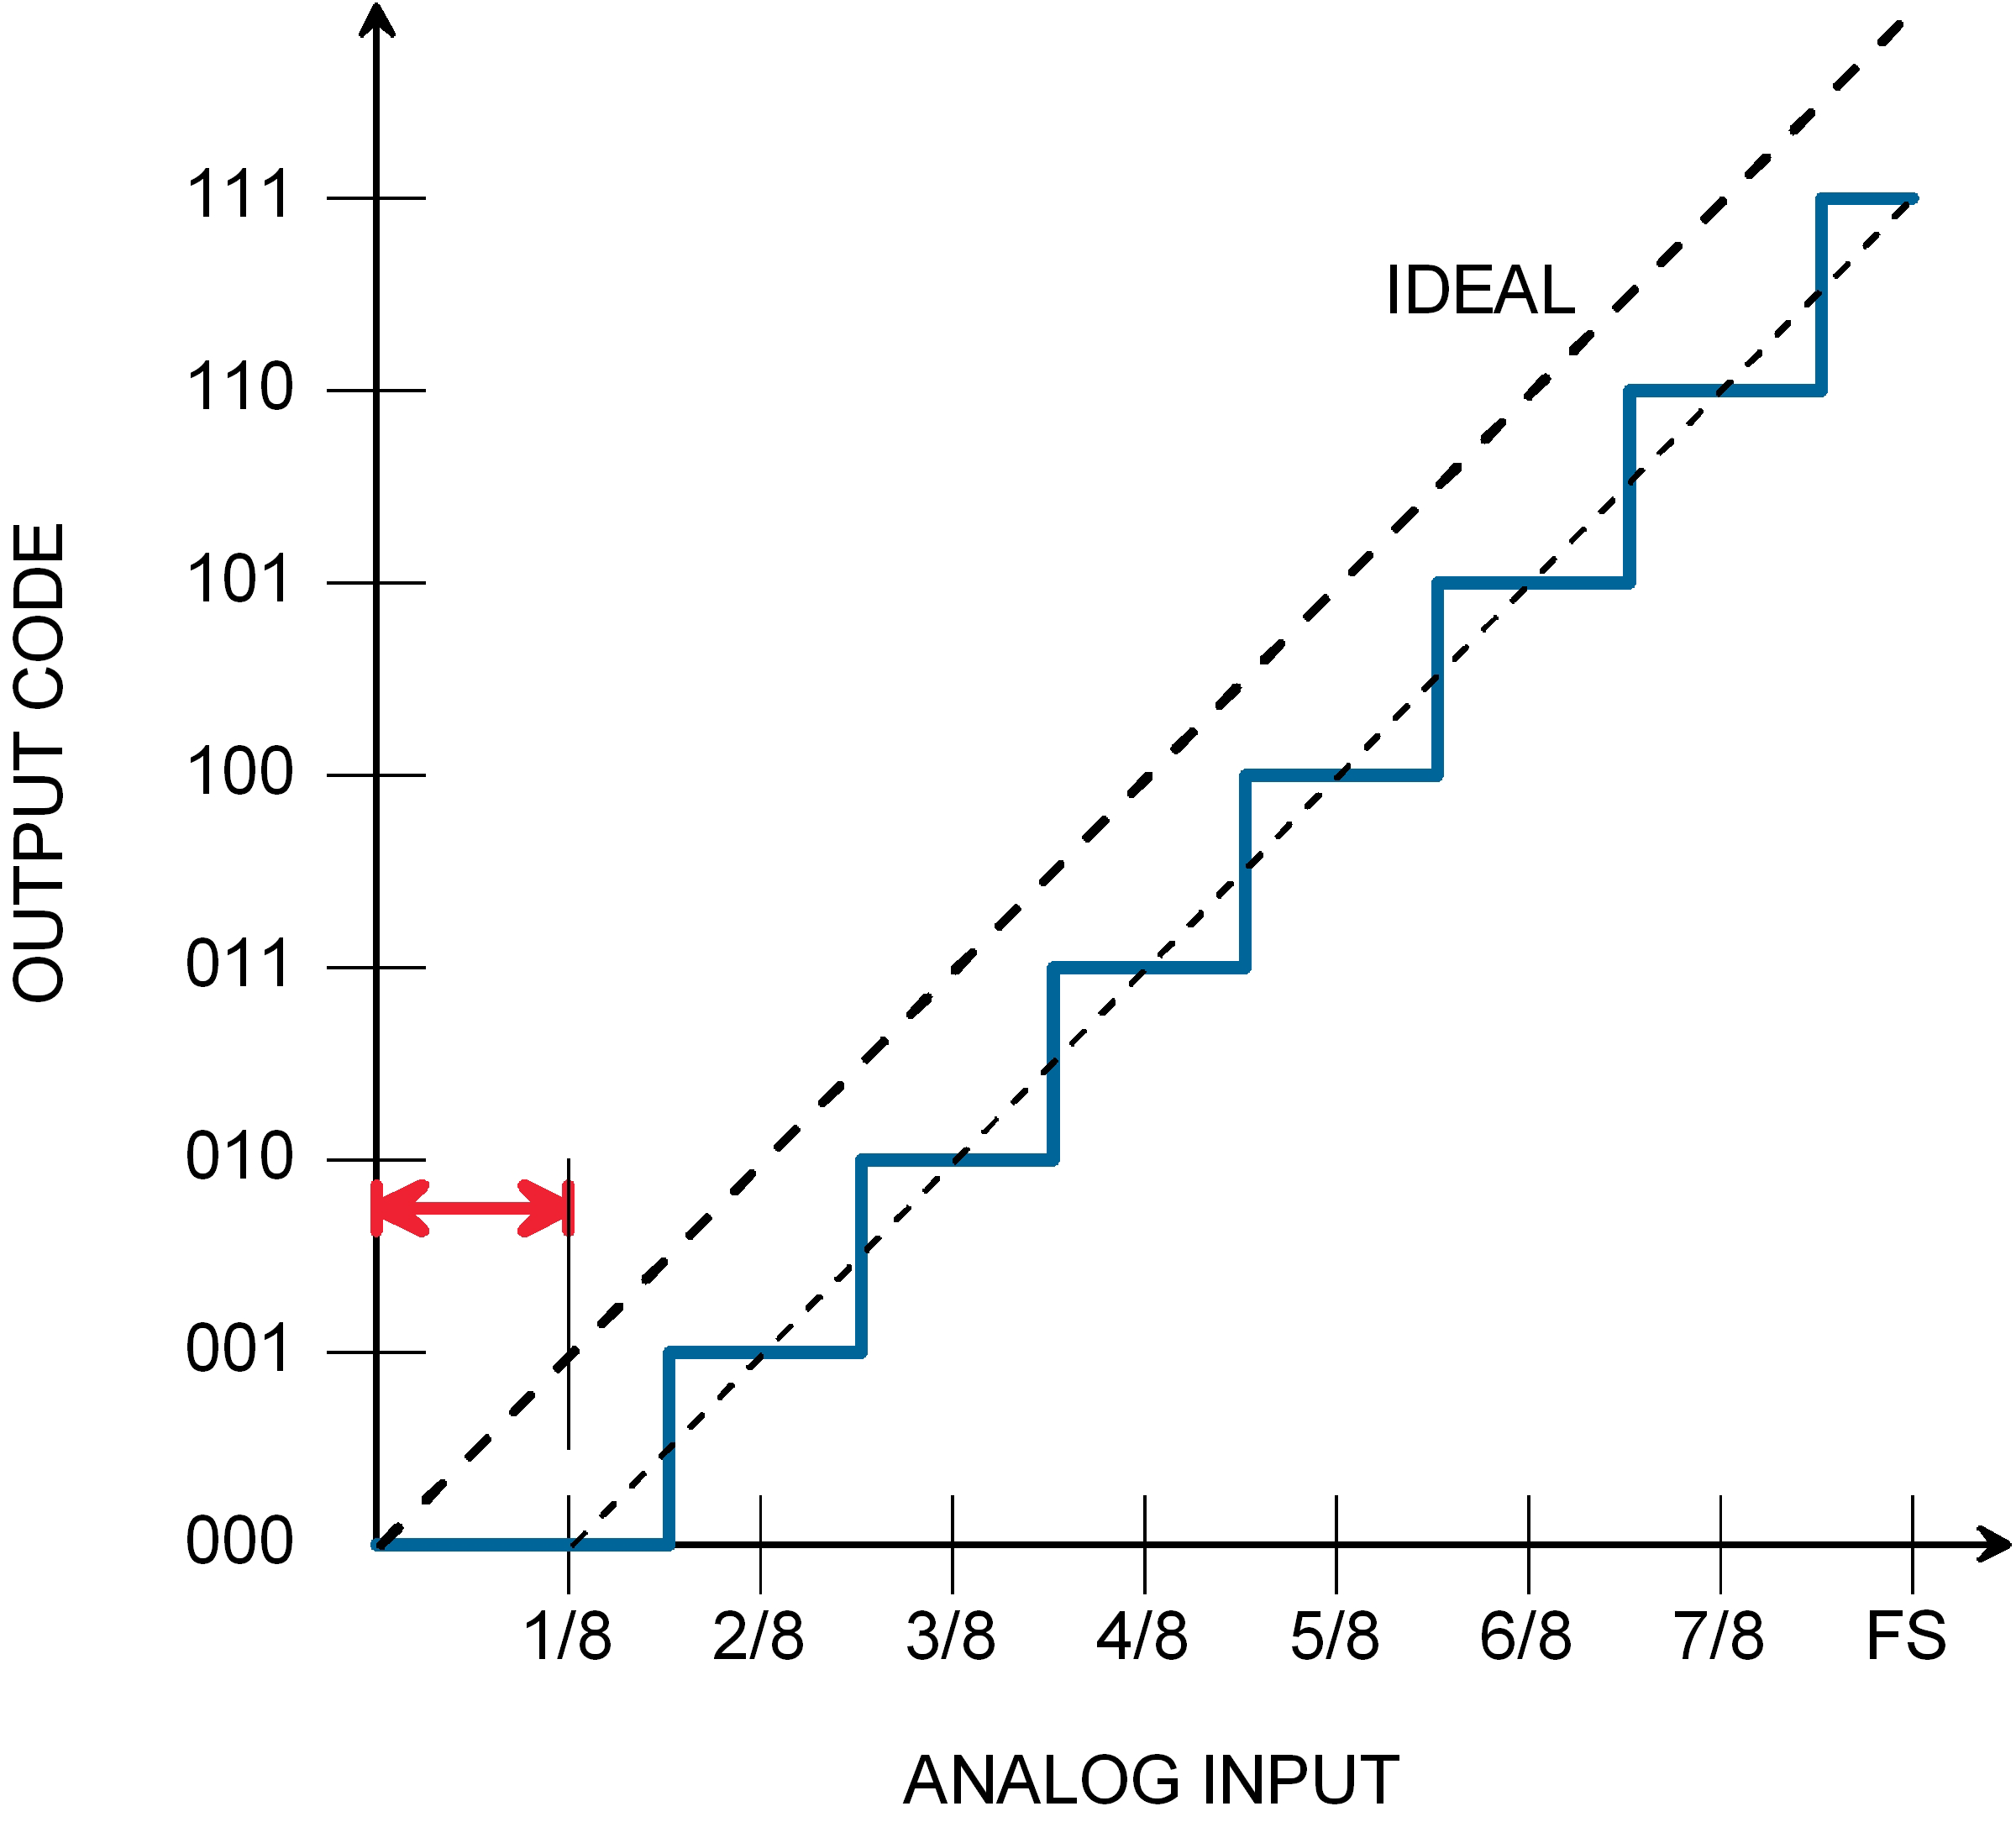
\includegraphics[
		width=0.25\textwidth,
		keepaspectratio,
		angle=0
		]{images/DacAdc/offset} & 
	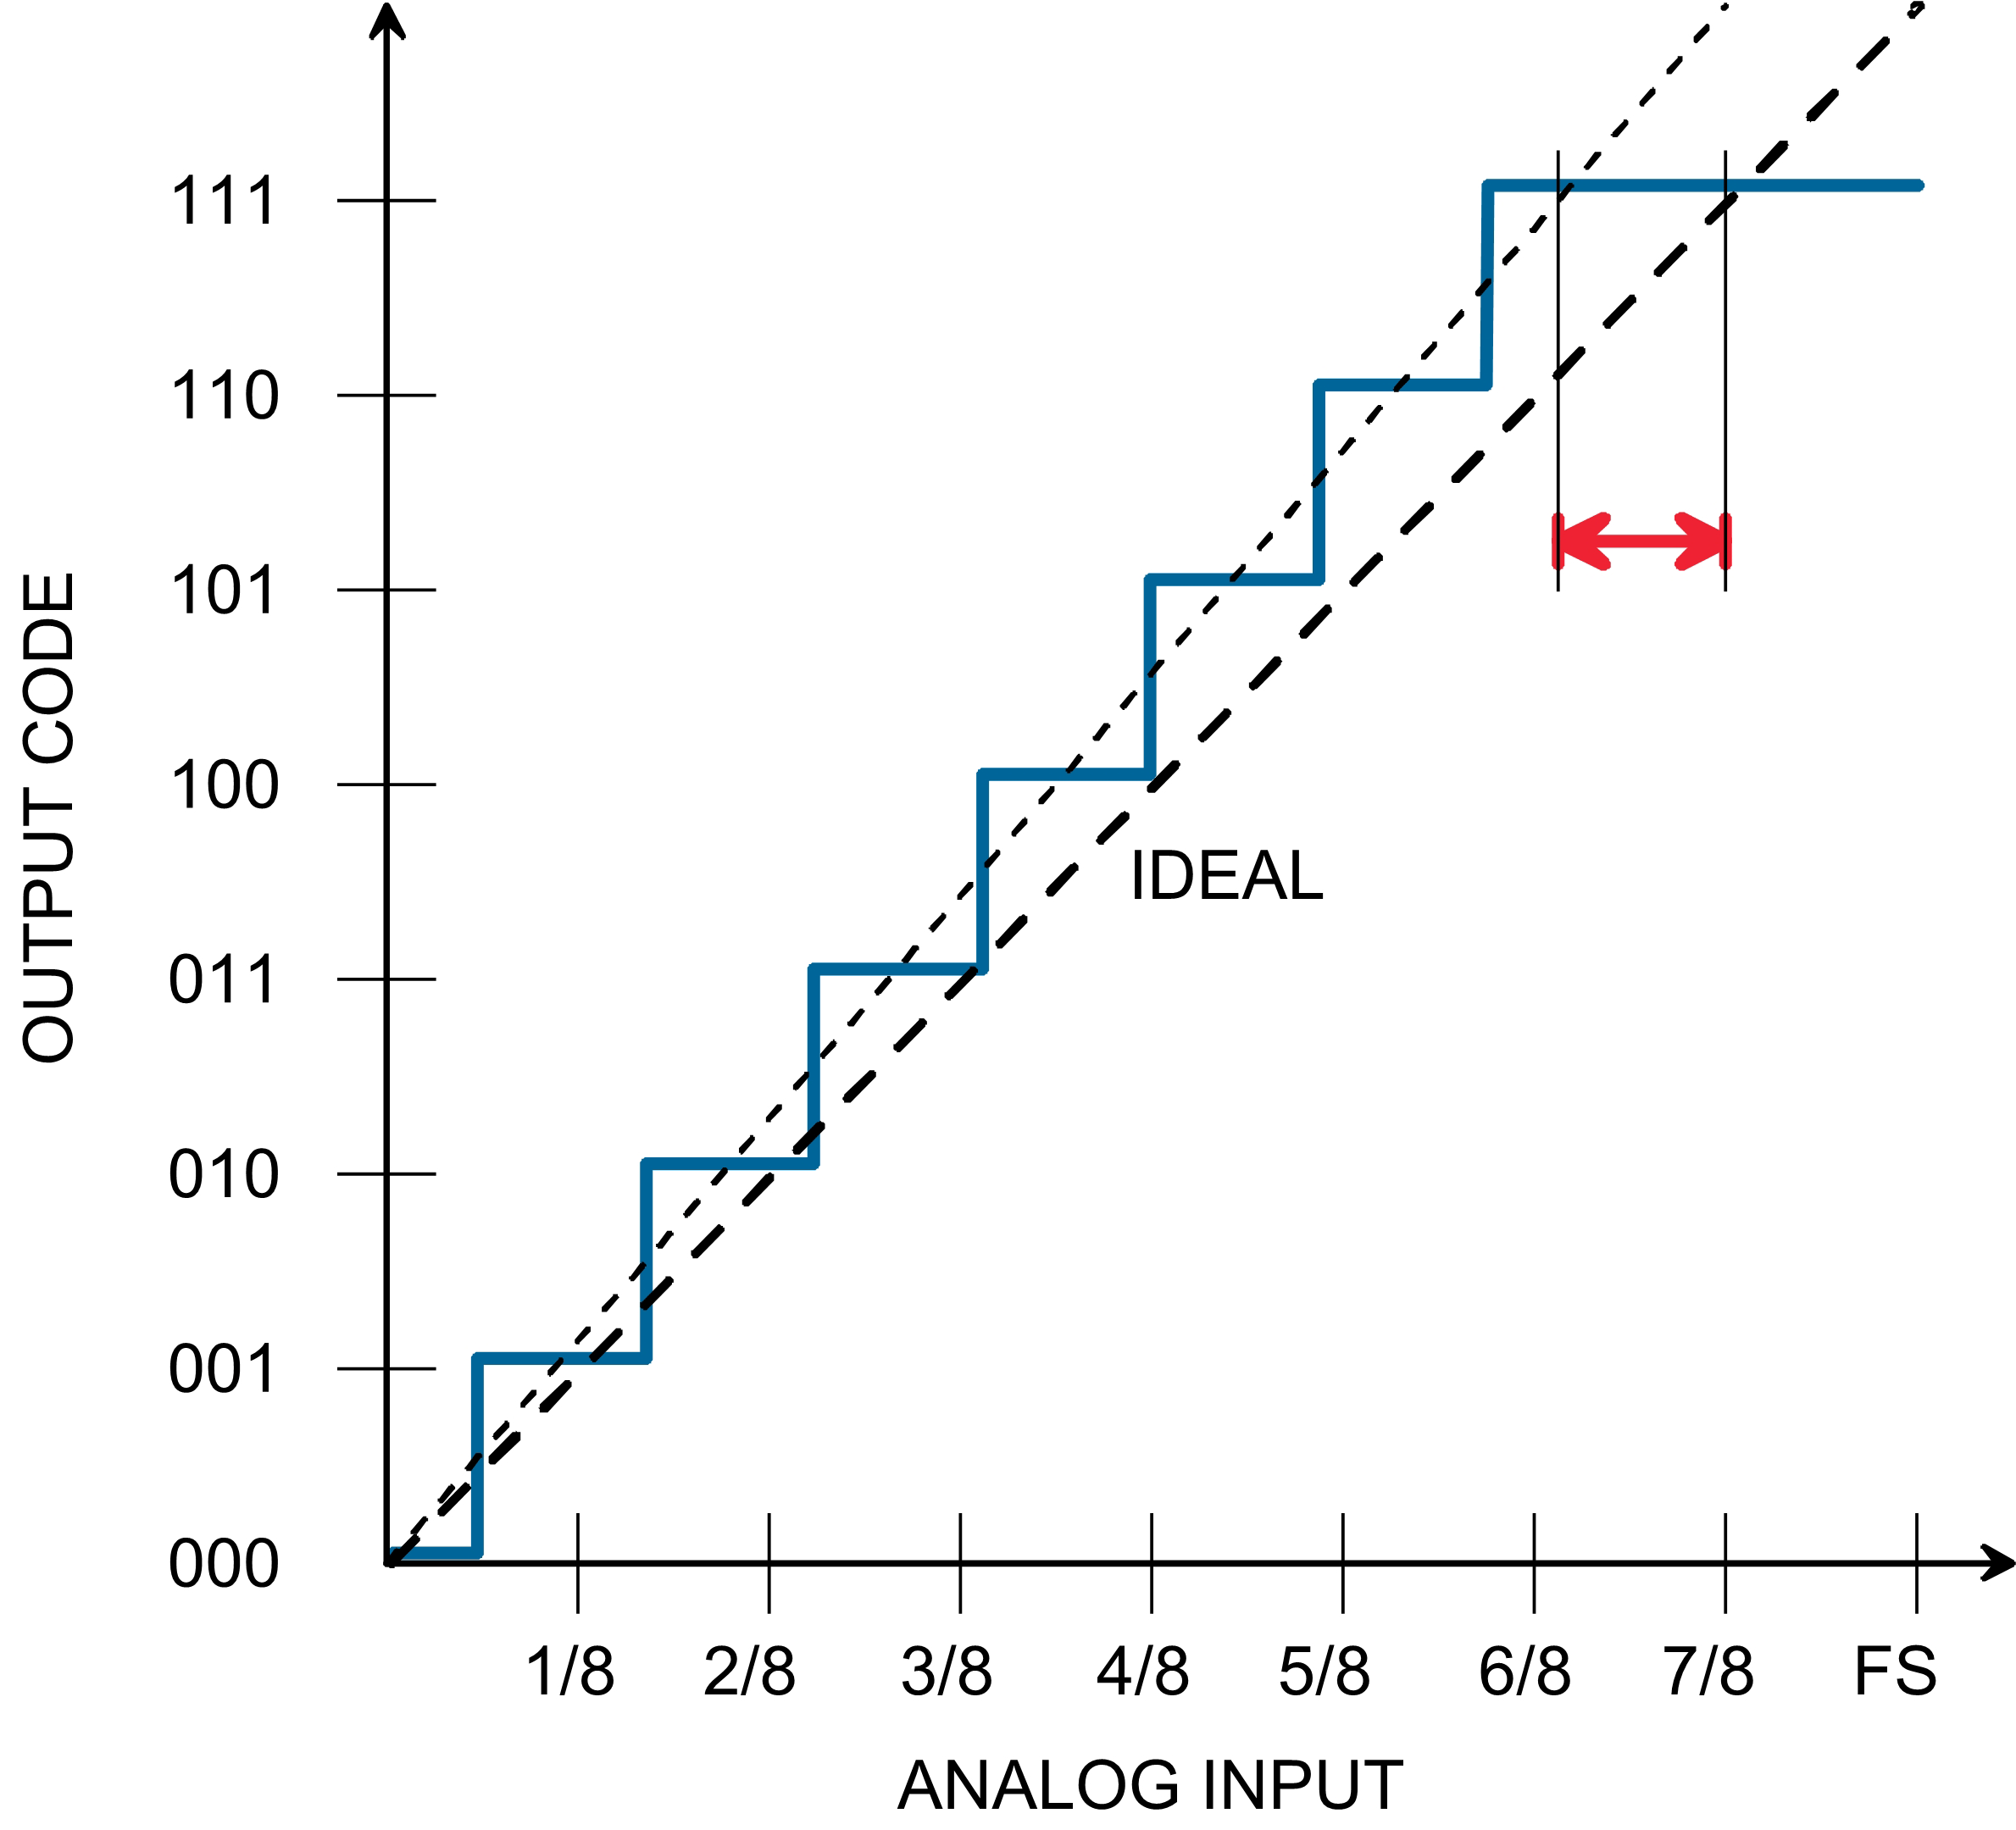
\includegraphics[
		width=0.25\textwidth,
		keepaspectratio,
		angle=0
		]{images/DacAdc/gain} & \\ 
		
	INL / DNL & Missing Codes & \\ 
	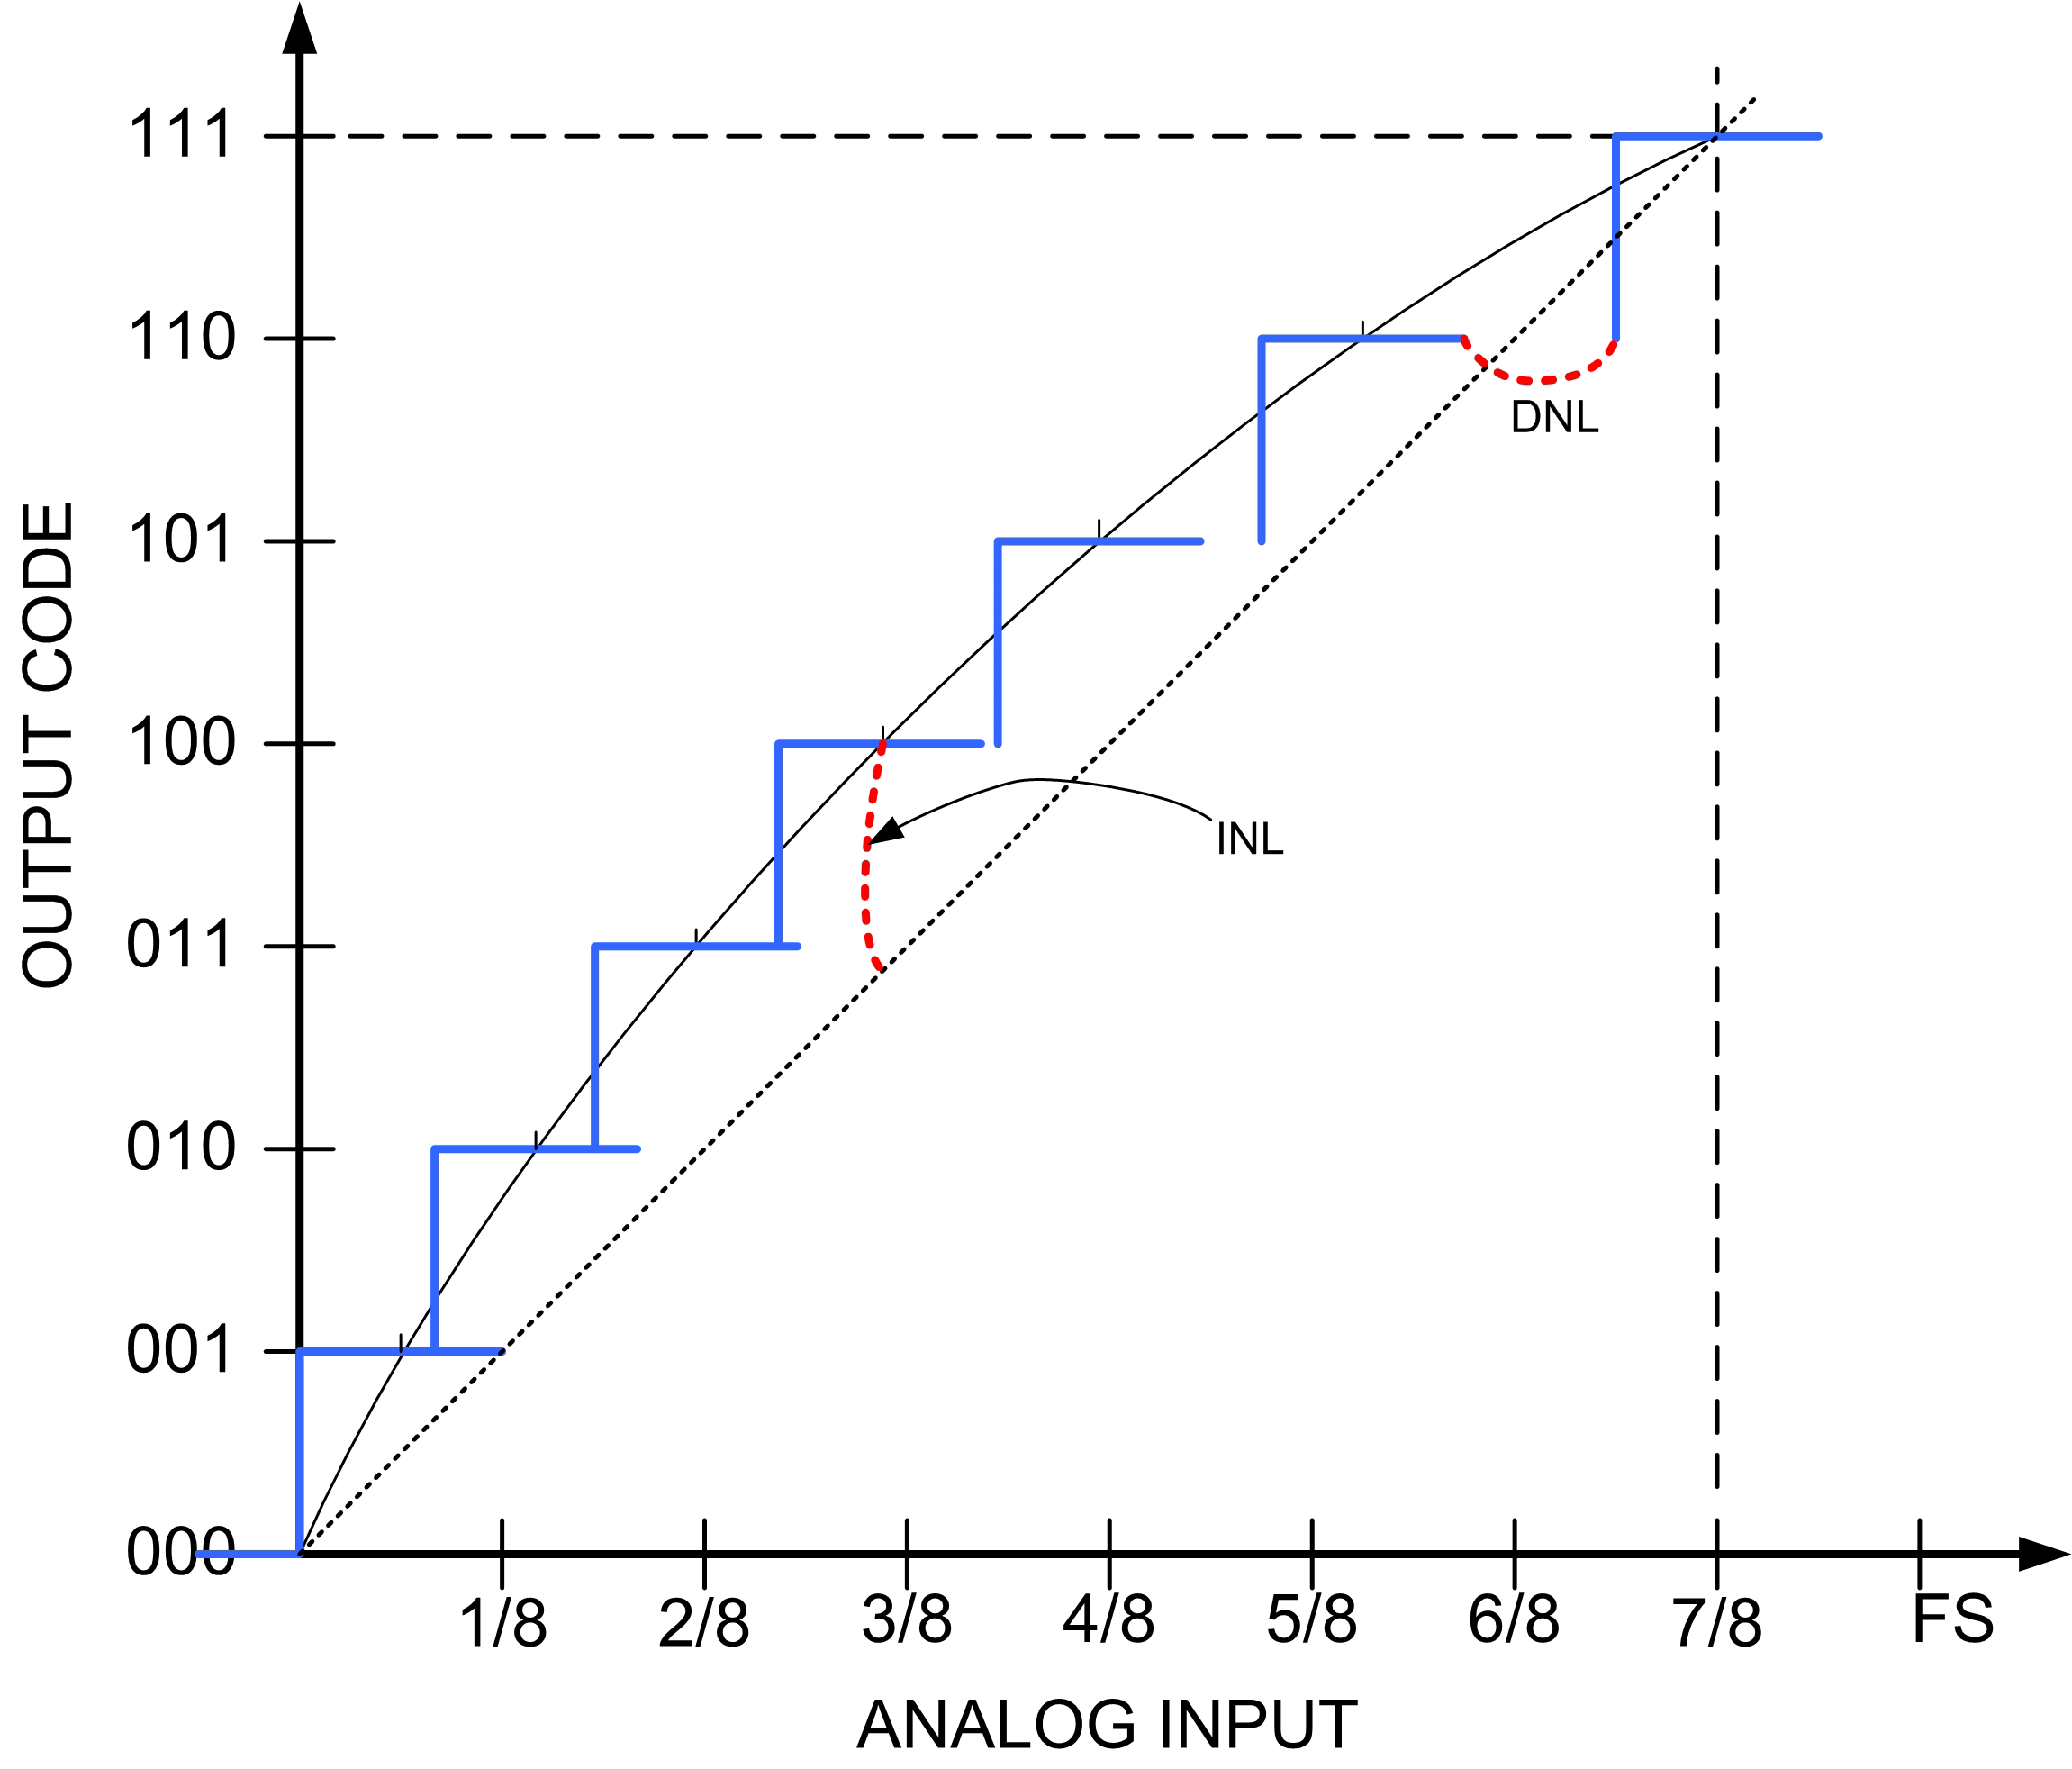
\includegraphics[
		width=0.25\textwidth,
		keepaspectratio,
		angle=0
		]{images/DacAdc/inl_dnl} & 
	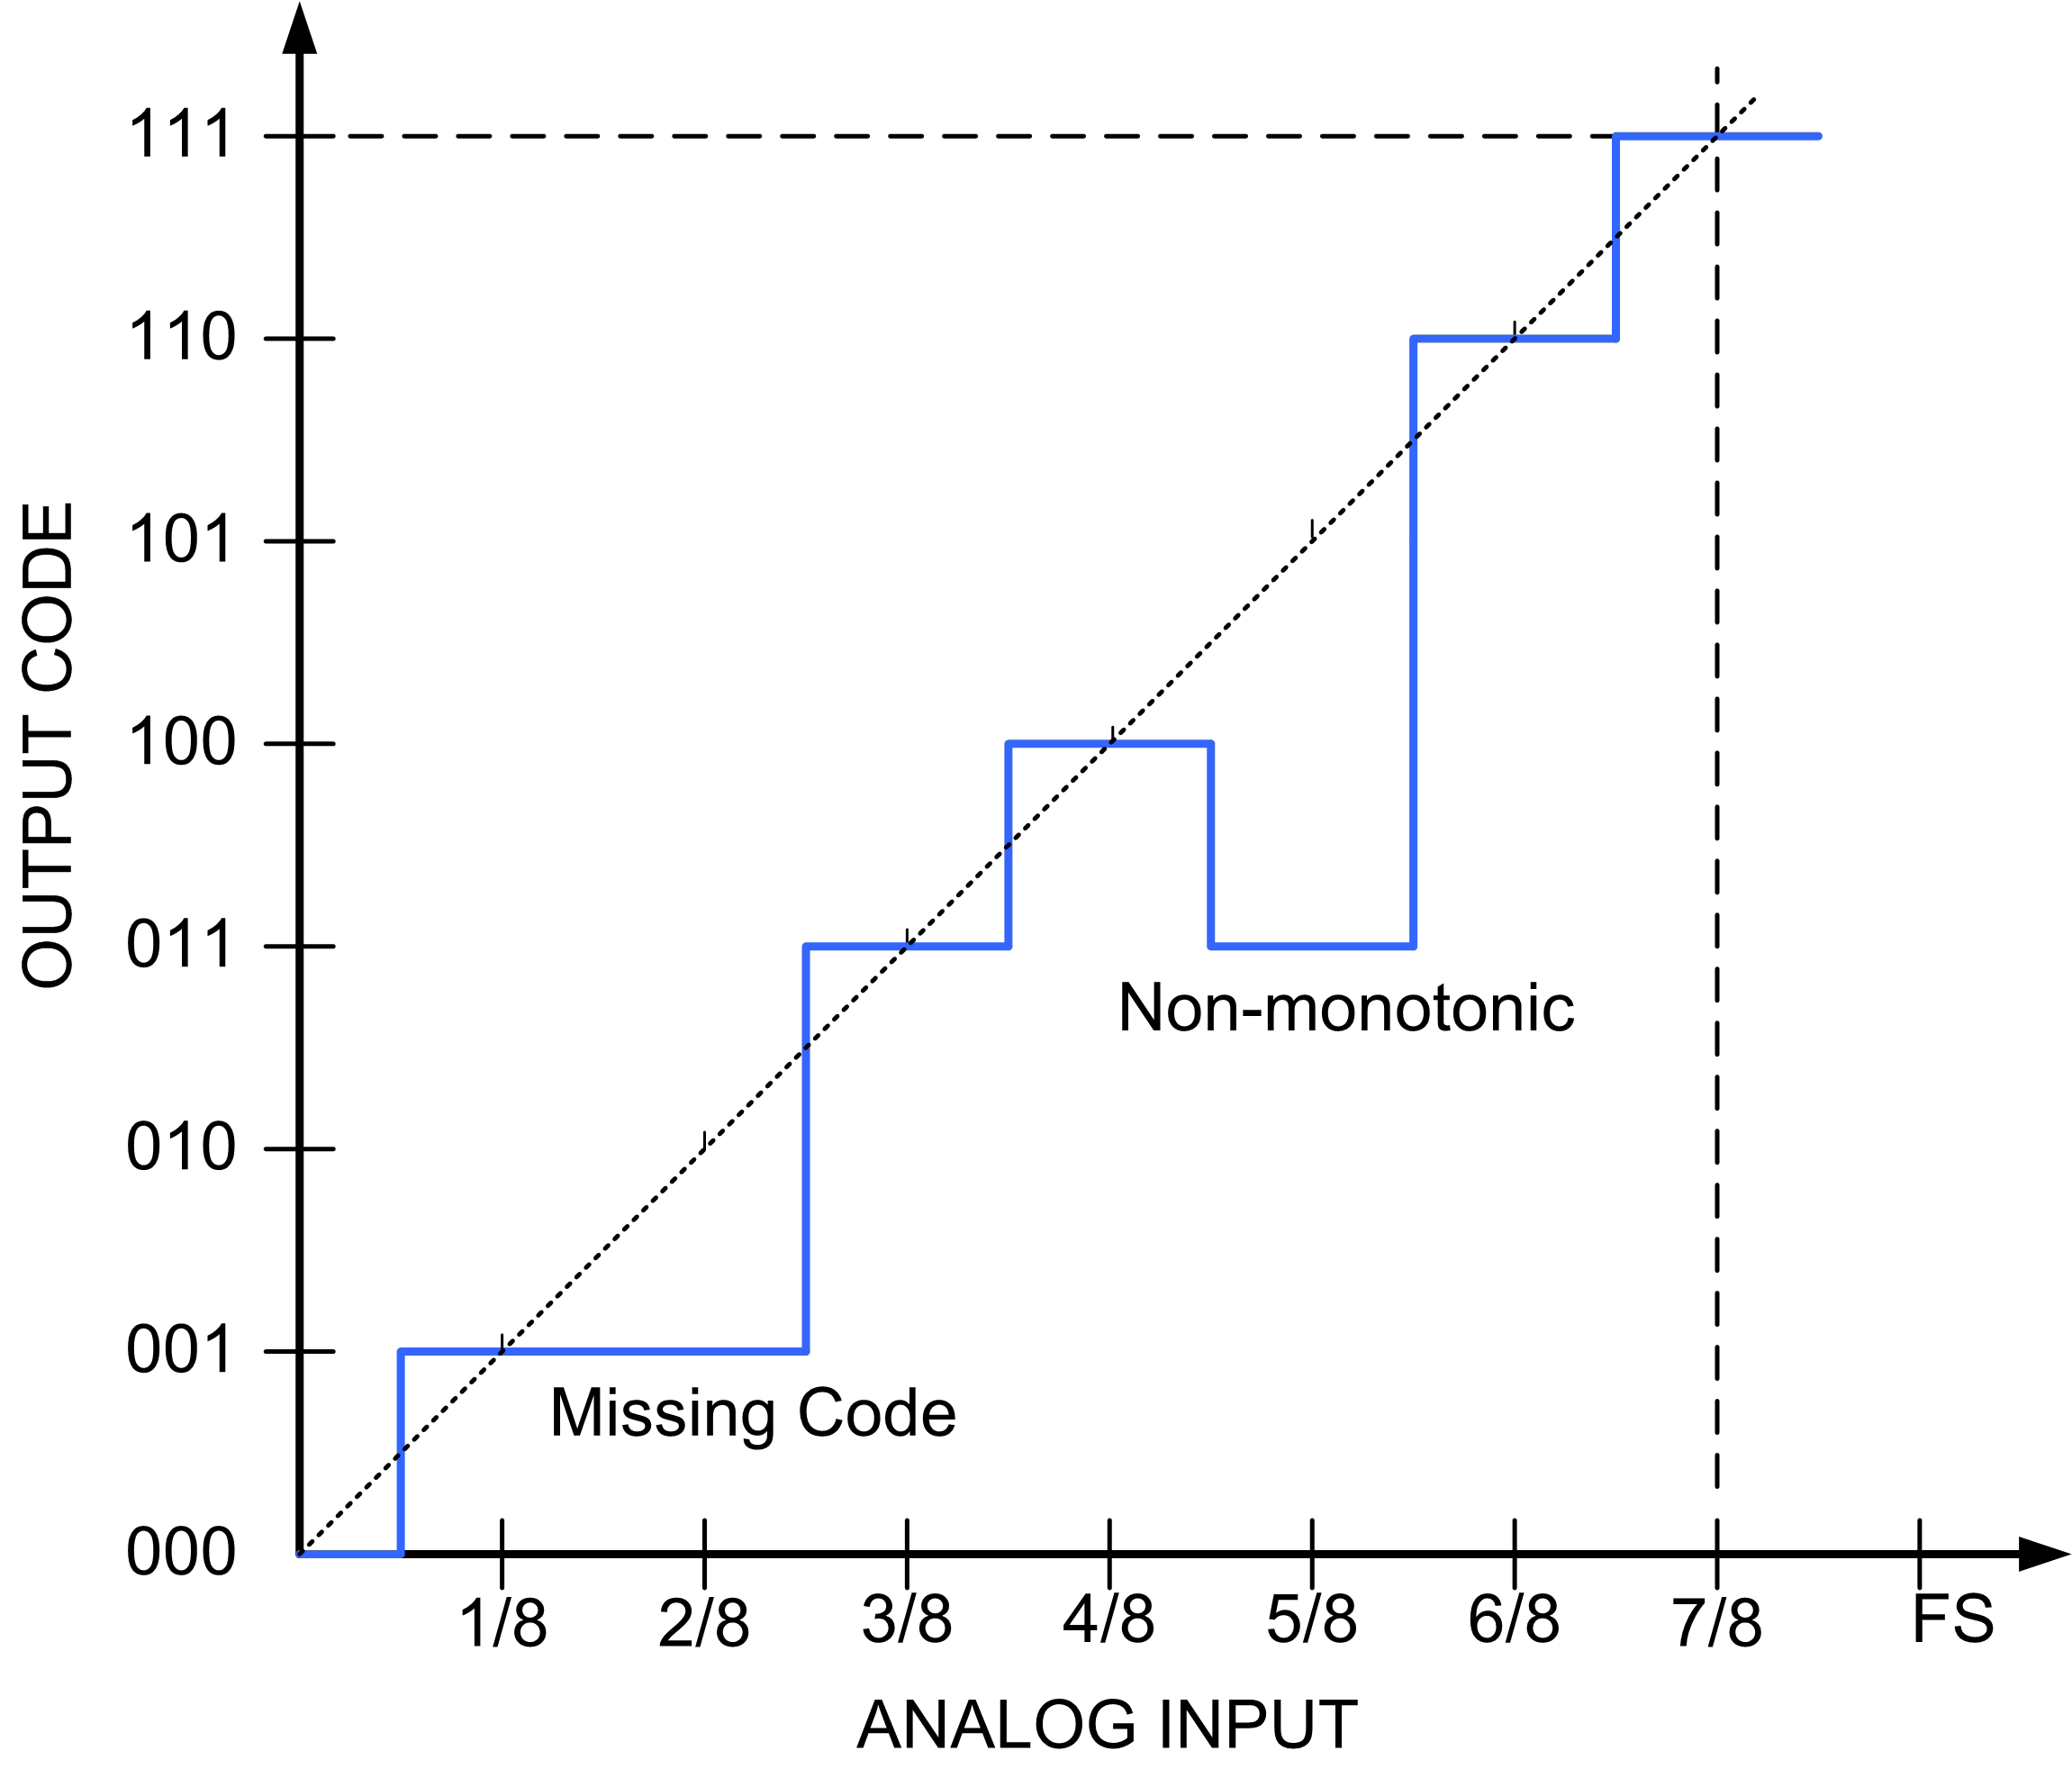
\includegraphics[
		width=0.25\textwidth,
		keepaspectratio,
		angle=0
		]{images/DacAdc/missing_codes} & 
		\begin{minipage}{0.4\textwidth}
		\begin{itemize}
			\item DNL $< -1$ $\rightarrow$ Non-monotonic
			\item DNL $> +1$ $\rightarrow$ Missing Code
		\end{itemize}
		\end{minipage}\\ 

\end{tabular}

\subsection{DAC}
Unitary: Monotonicity guaranteed but needs $2^N$ elements!

\begin{tabular}{m{8cm} m{6cm}}
 	Kelvin Divider & Segmented Chains \\ 
	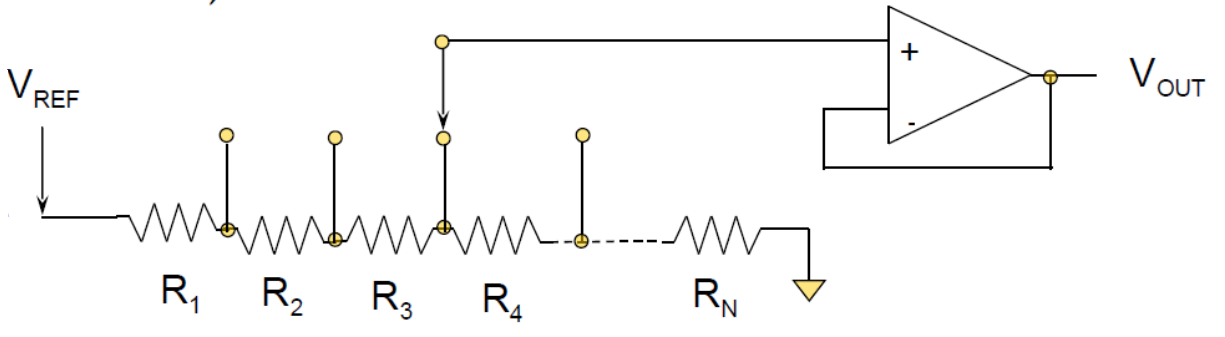
\includegraphics[
		width=8cm,
		keepaspectratio,
		angle=0
		]{images/DacAdc/kelvin_divider} & 
	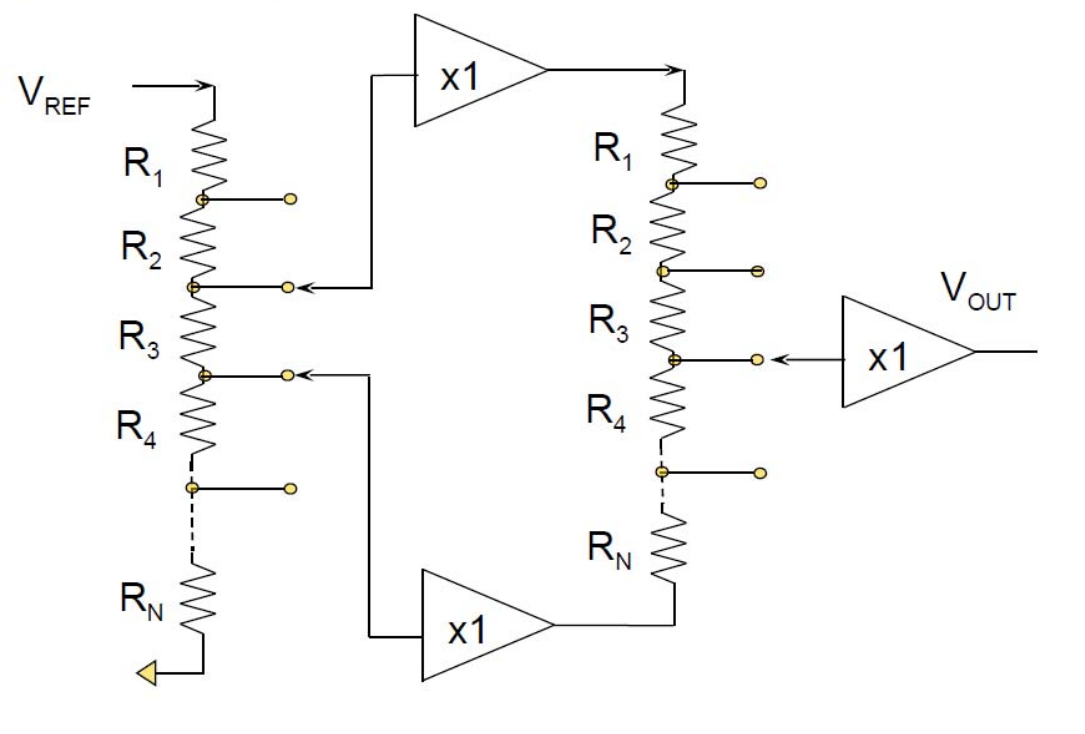
\includegraphics[
		width=6cm,
		keepaspectratio,
		angle=0
		]{images/DacAdc/segmented_chain} \\ 
\end{tabular}

Binary: No monotonicity guaranteed but needs just $N$ elements!

\begin{tabular}{m{8cm} m{8cm}}
 	Binary weighted & R-2R structure \\ 
	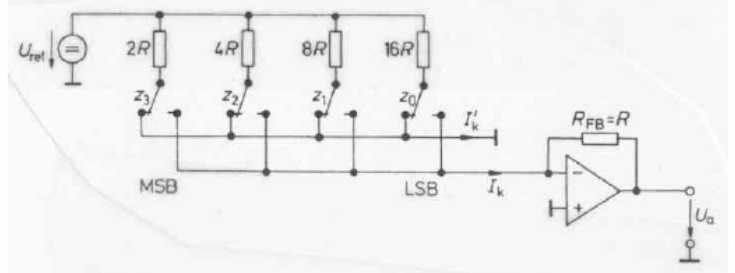
\includegraphics[
		width=8cm,
		keepaspectratio,
		angle=0
		]{images/DacAdc/binary_weighted} & 
	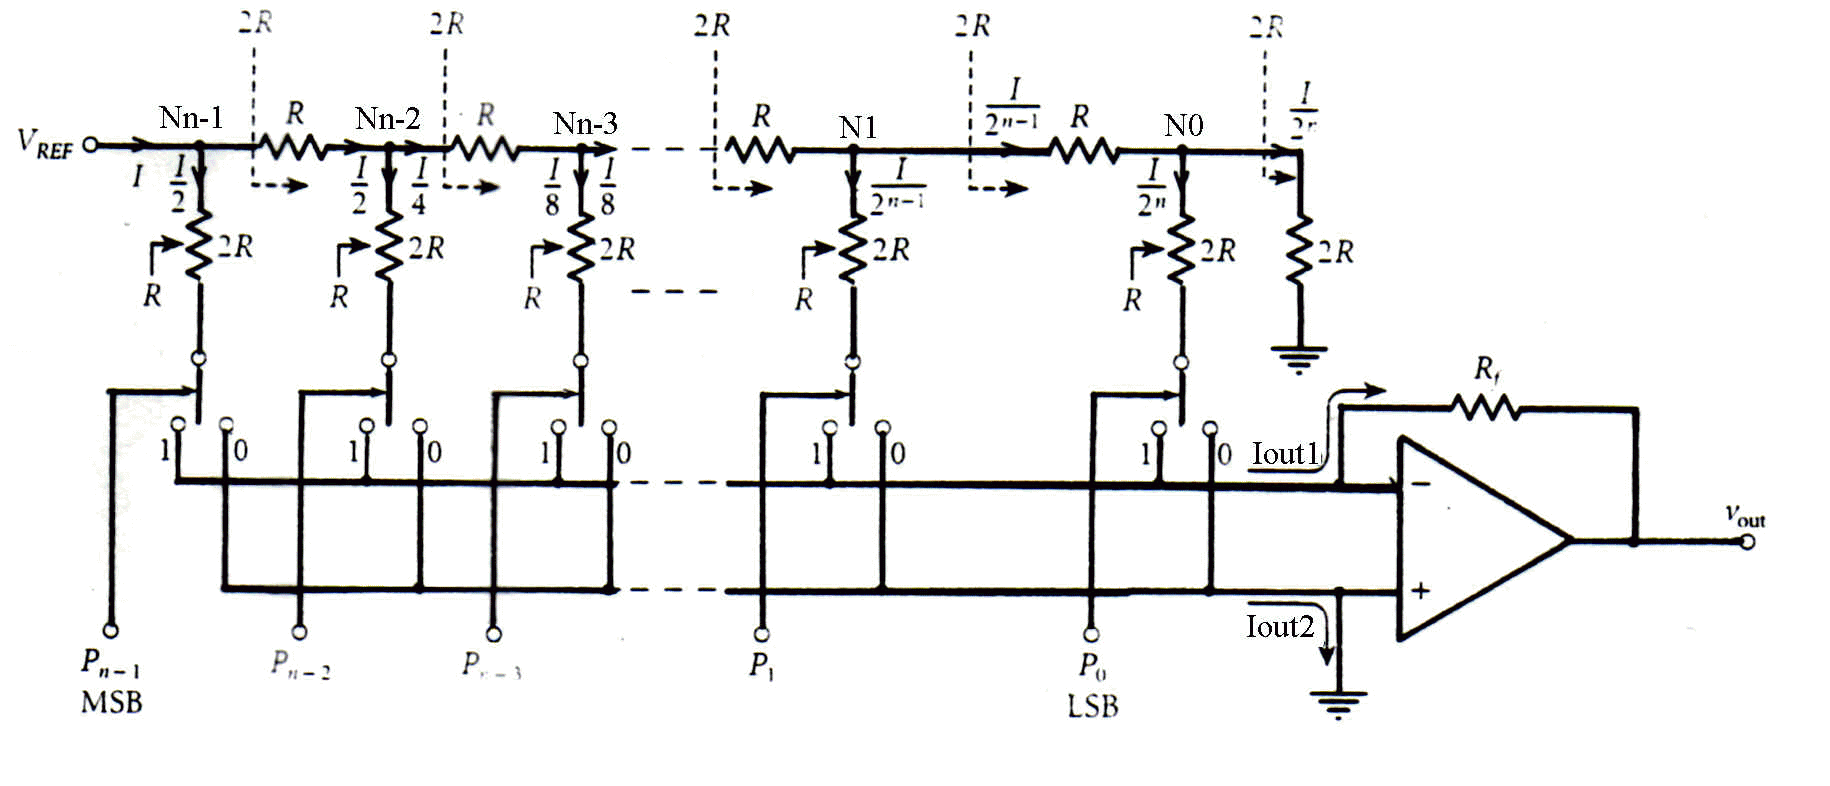
\includegraphics[
		width=8cm,
		keepaspectratio,
		angle=0
		]{images/DacAdc/r_2r} \\ 
\end{tabular}

\subsection{ADC}
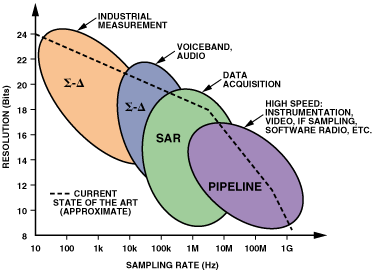
\includegraphics[
	width=8cm,
	keepaspectratio,
	angle=0
	]{images/DacAdc/samp_res} \\ 
	
\begin{tabular}{m{5cm} m{5cm}}
 	Flash: Fast 100M-1G / \quad High power / 6-8 Bits & Pipeline: Fast 1M-500M / High power / 8-12 Bits  \\ 
	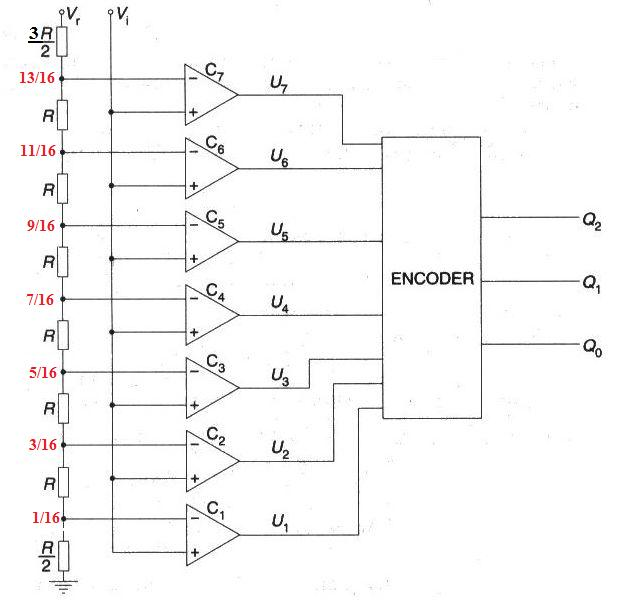
\includegraphics[
		width=5cm,
		keepaspectratio,
		angle=0
		]{images/DacAdc/flash} & 
	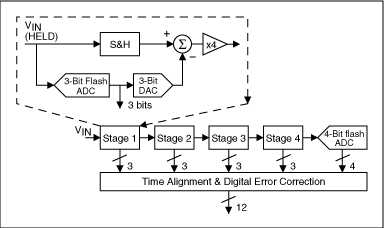
\includegraphics[
		width=5cm,
		keepaspectratio,
		angle=0
		]{images/DacAdc/pipelined}\\ 
		
	SAR: Medium 100K-10M / Medium power / 8-16 Bits & Sigma-Delta: Slow 10-100K / Low power / 14-24 Bits \\ 
	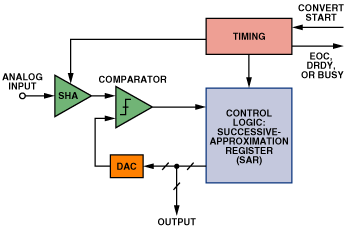
\includegraphics[
		width=5cm,
		keepaspectratio,
		angle=0
		]{images/DacAdc/sar} & 
	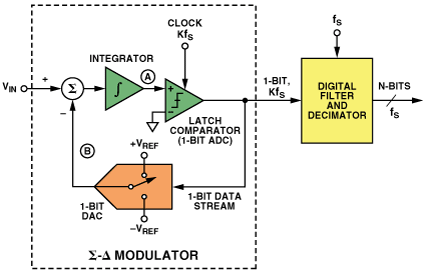
\includegraphics[
		width=5cm,
		keepaspectratio,
		angle=0
		]{images/DacAdc/sigma_delta}\\ 

\end{tabular}

Many ADC's have differential inputs. There are also differential opamp's to create the differential signals:
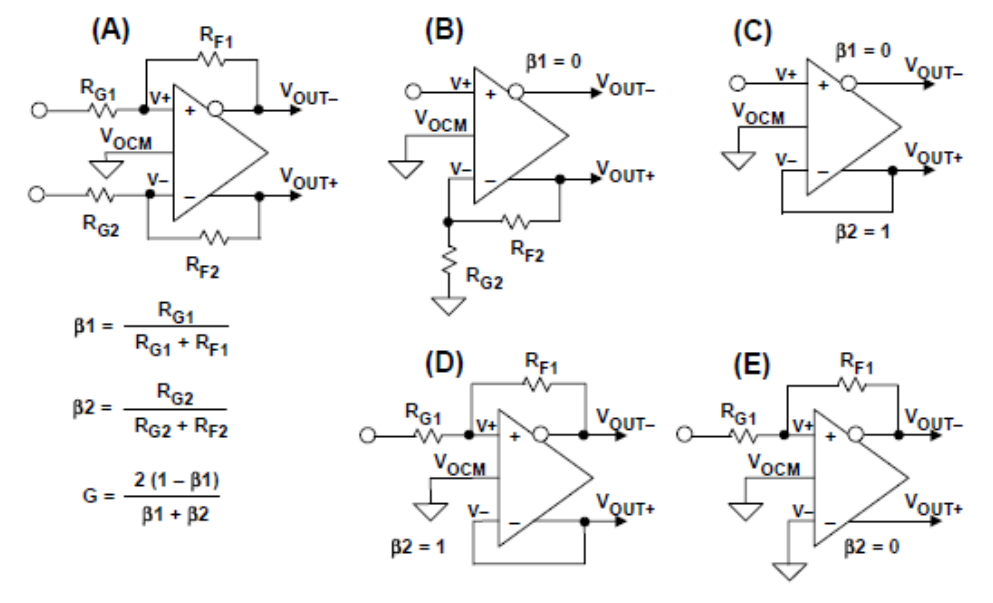
\includegraphics[
		width=0.5\textwidth,
		keepaspectratio,
		angle=0
		]{images/DacAdc/diff_amp}

\subsection{Sampling}
Normally, sampling is done using a Nyquist conversion: $f_s \geq 2f_{hi}$ If the signal is band limited on a high frequency, also undesampling is possible: $f_s \geq 2(f_{hi}-f_{lo})$\\
If the signal is band limited, noise can be removed by bandpass filtering the signal after the converter resulting in a higher $SNR_{db} = 1.76 + N \cdot 6.02 + 10 \cdot \log_{10}(\frac{f_s}{2 \cdot BW}) $\\

\newpage
\subsection{Oversampling}
Oversampling is done by sampling the signal faster than necessary: $f_s \geq OSR \cdot 2f_{hi}$ and then lowpass filtering the signal removing noise resulting in a higher $SNR_{db} = 1.76 + N \cdot 6.02 + 10 \cdot \log_{10}(OSR) $\\
Using oversampling and noise shaping (Sigma-Delta conversion) the SNR is future reduced:\\

\begin{tabular}{m{6cm} m{5cm} m{5cm}}
 	Principle & 1 Bit 1. Order & 1 Bit 2. Order \\ 
	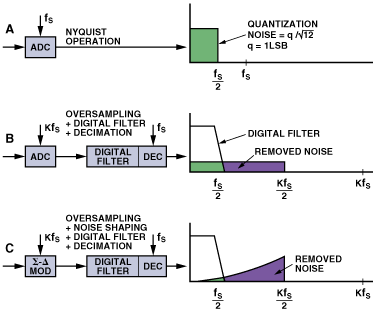
\includegraphics[
			width=6cm,
			keepaspectratio,
			angle=0
			]{images/DacAdc/oversampling} & 
	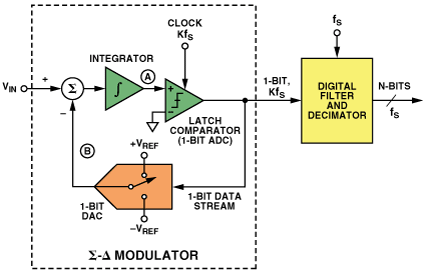
\includegraphics[
			width=5cm,
			keepaspectratio,
			angle=0
			]{images/DacAdc/sigma_delta} &
	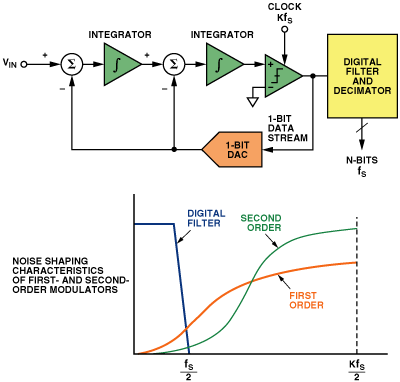
\includegraphics[
			width=5cm,
			keepaspectratio,
			angle=0
			]{images/DacAdc/sigma_delta_2ord} \\ 
\end{tabular}

%The formulas in the presentation are basicaly wrong, it is not (2*pi)^2 but 2 * pi^2 and so on...
\begin{tabular}{|c|c|c|c|c|}
\hline Order & 1 & 2 & 3 & L \\ 
\hline $\frac{N(z)}{E(z)}$ & $1-z^{-1}$ & $(1-z^{-1})^2$ & $(1-z^{-1})^3$ & $(1-z^{-1})^L$ \\ 
\hline Base-band noise voltage $n_0$ & $\frac{U_{LSB} \pi}{\sqrt{36}} \left( \frac{1}{OSR} \right)^{3/2} $ & $\frac{U_{LSB} \pi^2}{\sqrt{60}} \left( \frac{1}{OSR} \right)^{5/2}$ & $\frac{U_{LSB} \pi^3}{\sqrt{84}} \left( \frac{1}{OSR} \right)^{7/2} $ & $\frac{U_{LSB} \pi^L}{\sqrt{12(2L+1)}} \left( \frac{1}{OSR} \right)^{(2L+1)/2}$ \\ 
\hline SNR (Not in db!) & $\frac{9 \cdot OSR^3}{2\pi^2}$ & $\frac{15 \cdot OSR^5}{2\pi^4}$ & $\frac{21 \cdot OSR^7 }{2\pi^6}$ & $\frac{3}{2} \cdot \frac{(2L+1) \cdot OSR^{(2L+1)}}{\pi^{2L}}$  \\ 
\hline 
\end{tabular} 